\documentclass[aspectratio=169,t,xcolor=table]{beamer}
\usepackage[utf8]{inputenc}
\usepackage{footnote}
\usepackage{cite}
\usepackage{lipsum}
\usepackage{amsmath,amssymb,amsfonts}
\usepackage{graphicx}
\usepackage{textcomp}
\usepackage{xcolor}
\usepackage{graphicx}
\usepackage{booktabs}
\usepackage{dblfloatfix}
\usepackage{pgf,tikz,pgfplots}
\usepackage{bibentry}
\usepackage{etoolbox}
\usepackage{algorithm,algpseudocode}
%\usepackage[document]{ragged2e}
\usepackage{animate}
\usepackage{caption}
\usepackage{amsthm}
%\usepackage{subcaption}

% \usepackage{subfigure}
% \usepackage{hyperref}
% \usepackage{float}

% \usepackage{multicol}
% \usepackage{multirow}
 \usepackage{etoolbox}\AtBeginEnvironment{algorithmic}{\tiny}
\usetheme{Ufg}

%\algsetup{linenosize=\tiny}
%----------------------- Primary Definitions -----------------%

% This command set the default Color, is also possible to choose a custom color
\setPrimaryColor{DarkGreen} 
% First one is logo in title slide (we recommend use a horizontal image), and second one is the logo used in the remaining slides (we recommend use a square image)
\setLogos{lib/logos/logoHDSP2.png}{lib/logos/logo_uis_cuadro.png}


% If second logo for another academic institution use the following command
% \setAuxiliarLogo{lib/logos/stsiva_logo.png}

% -------------------------------------- Title Slide Information
\DeclareMathOperator*{\minimize}{minimizar} % Declaración operador minimize

\DeclareMathOperator*{\maximize}{maximizar} % Declaración operador maximize
\DeclareMathOperator*{\subjectto}{sujeto \ a} % Declaración operador subjectto
\DeclareMathOperator*{\argmax}{arg \ max} % Declaración operador arg max
\DeclareMathOperator*{\argmin}{arg \ min}
%\DefineBibliographyStrings{spanish}{andothers={et~al\adddot}}
% Traducción de palabras reservadas del algoritmo a español

\renewcommand{\algorithmname}{Algoritmo}%
\renewcommand{\algorithmicif}{\textbf{si}}%
\renewcommand{\algorithmicthen}{\textbf{entonces}}%
\renewcommand{\algorithmicend}{\textbf{fin}}%
\renewcommand{\algorithmicfor}{\textbf{para}}%
\renewcommand{\algorithmicdo}{\textbf{hacer}}%



\begin{document}
\title[Inf UFG]{Algoritmo de clasificación de objetos en imágenes difractivas basado en medidas cuadráticas codificadas usando un enfoque de aprendizaje profundo}
\subtitle{Trabajo de Grado para optar al título de Ingeniero de Sistemas.}
\author{Autor: David Santiago Morales Norato \\ Director: Phd(c) Andrés Jerez \\ Codirector: Phd. Henry Arguello}

\institute[UFG] % (optional)
{
  \inst{}Escuela de Ingeniería de Sistemas e Informática,\\ \textit{Universidad Industrial de Santander}, Bucaramanga, Colombia
}
\date{\vspace{1cm}2022}
%-----------------------The next statement creates the title page.
\frame[noframenumbering]{\titlepage}

%---------------------------------------------------------
\setLayout{vertical} % This command define the layout. 'vertical' can be replace with 'horizontal', 'blank, 'mainpoint', 'titlepage'

%Outline is updated automatically once you add a section, subsection or a subsubsection

% \begin{frame}
%     \scriptsize
%     \frametitle{Agenda del día}
%     \tableofcontents
% \end{frame}
%---------------------------------------------------------


\section{Motivación}
\subsection{Aplicaciones de medidas cuadráticas}
\begin{frame}{Aplicaciones de medidas cuadráticas }
    \centering
    \scriptsize
    \animategraphics[loop,autoplay,width=0.5\linewidth]{1}{gifs/applications-}{0}{8}
\end{frame}
% \subsection{Clasificación de imágenes de sistemas lineales}
% \begin{frame}{Clasificación de imágenes de sistemas lineales}
% \scriptsize
% \centering
%         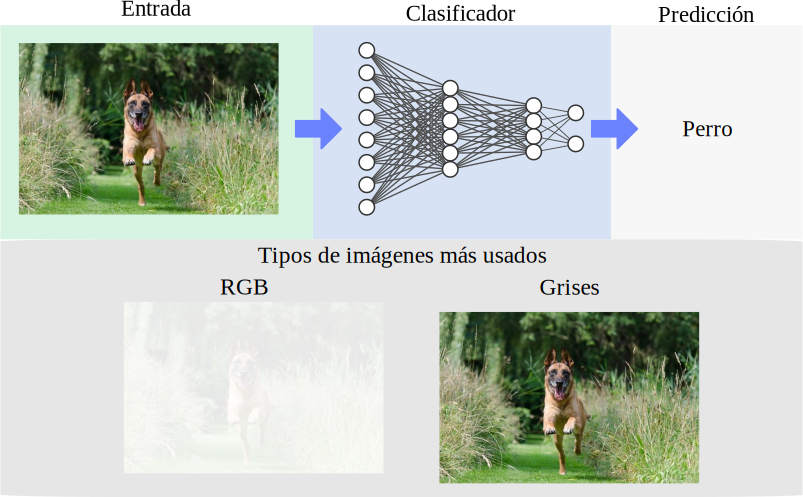
\includegraphics[width=0.6\linewidth]{images/marco_teórico/clasificacion.pdf}\

%       \begin{block}{\scriptsize  Modelo de adquisición.}
%         \vspace{-0.3cm}
%         %\vspace{-1cm}
%         \begin{equation}
%             \mathbf{y}= \mathbf{A}\mathbf{z}, 
%         \end{equation}

%       \end{block}
%         \begin{itemize}
%         \item $\mathbf{y}\in\mathbb{R}^n$: medidas lineales
%          \item $\mathbf{z}\in \mathbb{R}^{n}$: Escena
%         \end{itemize}
%     \begin{itemize}
%         \item $\mathbf{A}$ Representa la matriz de sensado del sistema óptico
%     \end{itemize}


% \end{frame}

\subsection{Adquisición de la información de fase}

\begin{frame}{Imágenes Difractivas}
\scriptsize
\centering
%\vspace{-4mm}

    \includegraphics[width=0.6\linewidth]{images/marco_teórico/diffraction_no_coded.pdf}%\vspace{-3mm}
    \begin{columns}
    \column{0.6\linewidth}
        
       \begin{block}{\scriptsize  Modelo de propagación.}
        %\vspace{-0.3cm}
        \vspace{-1cm}
        \begin{equation}
            \mathbf{y}_{\psi}= \vert \mathbf{A}_\psi \mathbf{z} \vert^2, \quad \mathbf{A}_\psi = \left\{\begin{matrix}
                     \mathbf{F}\mathbf{T}\mathbf{F}^\mathcal{H}    &  \psi=1\rightarrow \text{Cercano}\\ 
                     \mathbf{F}^\mathcal{H}\mathbf{Q} & \psi=2\rightarrow\text{Medio} \\ 
                     \mathbf{F}  & \psi=3\rightarrow\text{Lejano}
                    \end{matrix}\right.,
            \label{eq:diffraction_base}
        \end{equation}

       \end{block}
        \begin{itemize}
        
         \item $\mathbf{z}\in \mathbb{C}^{n}$: Escena
         
        \end{itemize}
    \column{0.48\linewidth}

    \begin{itemize}
        \item $\mathbf{Q}, \mathbf{T} \in \mathbb{C}^{n \times n}$ Funciones de transferencia del campo medio y cercano.
        %\item $(\mathbf{Q})_{p,q}=e^{\frac{-jk_0}{2z}(p^2\delta_x^2+q^2\delta_y^2)},$
        %\item $(\mathbf{T})_{r,s}=e^{-jk_0z\sqrt{1-\frac{(r\delta_{kx})^2}{k_0^2}-\frac{(s\delta_{ky})^2}{k_0^2}}}.\label{eq:Tfuncion}$
        \item $\mathbf{F}\in\mathbb{C}^{n\times n}$: transformada discreta de fourier.
        \item $\mathbf{y}_\psi\in\mathbb{R}^n$: medidas cuadráticas
        %\item  $k_0=2\pi/\lambda$: número de onda.
    \end{itemize}
\end{columns}
\end{frame}

\subsection{Medidas cuadráticas codificadas}

\begin{frame}{Medidas cuadráticas codificadas}
\scriptsize
\centering\vspace{-4mm}
        \includegraphics[width=0.6\linewidth]{images/marco_teórico/diffraction_coded.pdf}\vspace{-3mm}
    \begin{columns}
    \column{0.58\linewidth}
        
       \begin{block}{\scriptsize  Modelo de propagación.}
        %\vspace{-0.3cm}
        \vspace{-1cm}
        \begin{equation}
             \mathbf{y}_{\ell, \psi} = \vert \mathbf{A}_{\ell, \psi}\mathbf{z} \vert^2, \quad \mathbf{A}_{\ell,\psi}= \left\{\begin{matrix} \mathbf{F}\mathbf{T}\mathbf{F}^\mathcal{H} \mathbf{D}_\ell  & \psi=1\\                 \mathbf{F}^\mathcal{H}\mathbf{Q}\mathbf{D}_\ell & \psi=2 \\ 
                \mathbf{F}\mathbf{D}_\ell1  &\psi=3
                \end{matrix}\right..
            \label{eq:diffraction_base}
        \end{equation}

       \end{block}
        \begin{itemize}
        \item $\mathbf{y}_{\ell, \psi}$ medidas cuadráticas codificadas en la $\ell$-ésima proyección en el campo $\psi$, con, $\ell=\{1,\dots,L\}$
        \item $\mathbf{A}_{\ell, \psi}\in\mathbb{C}^{n\times n}$ matriz de sensado en la $\ell$-ésima proyección en el campo $\psi$,
        \end{itemize}
    \column{0.5\linewidth}
    \begin{itemize}
    \item $\mathbf{D}_{\ell} = \mathrm{diag}(\mathbf{d})$ son $i.i.d$, con $\mathbf{d} \in \{d\}^{n}$.
    \end{itemize}
    % Please add the following required packages to your document preamble:
    % \usepackage{graphicx}
    \begin{table}[]
    \centering
    \renewcommand*{\arraystretch}{1.5}
    \resizebox{0.8\textwidth}{!}{%
    \begin{tabular}{|c|c|}
    \hline
    Elemento de codificación & probabilidad                     \\ \hline
    $d \in \{0, 1\}$         &  $\{ \frac{1}{2},  \frac{1}{2}\}$ \\ \hline
    $d \in \{-1, 1\}$        & $\{ \frac{1}{2},  \frac{1}{2}\}$ \\ \hline
    $d \in \{-1, 1, -j,  j\}$ & $\{ \frac{1}{4},  \frac{1}{4}, \frac{1}{4},  \frac{1}{4}\}$ \\ \hline
    \end{tabular}%
    }
    \label{tab:comp_class_models}
    \end{table}
\end{columns}
\end{frame}


\subsection{Recuperación de la fase}
\begin{frame}{Recuperación de la fase \footnote{\tiny Jerez, A et al, (2020) "Fast Target Detection via Template Matching in Compressive Phase Retrieval"}}
\scriptsize
\vspace{-1cm}
\begin{block}{\scriptsize Formulación no convexa}
\centering
    \vspace{-1cm}
    \begin{equation}
    \small
    \hat{\mathbf{z}} \in \argmin_{{\mathbf{z}}\in\mathbb{C}^n}\Vert\mathbf{y}_{\psi} - \vert \mathbf{A}_{\psi}\mathbf{z} \vert^2\Vert_2^2, 
        \label{eq:phase_retrieval_problem}
    \end{equation}
    %\vspace{0.1cm}
\end{block}
\vspace{-1cm}
\begin{block}{\scriptsize Distancia}
\centering
    \vspace{-1cm}
    \begin{equation}
    \small
    \mathrm{dist}(\mathbf{z}, \hat{\mathbf{z}}) = \min_{\theta \in [0, 2\pi)}\Vert \mathbf{z}e^{-j\theta} - \tilde{\mathbf{z}}\Vert_2.
    \end{equation}
\end{block}

\vspace{0.5cm}

\noindent{%
\begin{minipage}[t]{0.4\linewidth}
    \begin{block}{\scriptsize Algoritmos de reconstrucción}
        \begin{itemize}
            \item \textit{Truncated Wirtinger Flow} (TWF).
            \item \textit{Truncated Amplitud Flow} (TAF) .
            \item \textit{Reweighted Amplitud Flow} (RAF).
        \end{itemize}
    \end{block}
\end{minipage}}%
\hfill%
{%
\begin{minipage}[t]{0.55\linewidth}
    \begin{block}{\scriptsize Algoritmos de inicialización}
        \vspace{-0.2cm}
        \hspace{2cm}
        \begin{itemize}
    
            \item \textit{Truncated Spectral Initialization} (TSI).
            \item \textit{Orthogonality promoting initialization} (OPI).
            \item \textit{Weighted Maximal Correlation Initialization} (WMCI).
            \item \textit{Filtered Spectral Initialization} (FSI).
        \end{itemize}
    \end{block}
\end{minipage}}


\end{frame}






\subsection{Enfoque de clasificación tradicional}
\begin{frame}{Clasificación de medidas cuadráticas}
\scriptsize

Clasificación de medidas cuadráticas de células. Adaptado de \footnote{\tiny Kim, S., et al. (2018). "Deep transfer learning-based hologram classification for molecular diagnostics".} 
    \begin{figure}
        \centering
        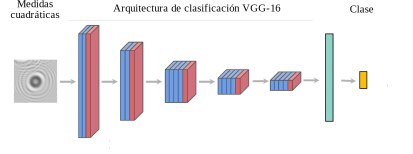
\includegraphics[height=0.35\textheight]{images/marco_teórico/cell_clasification.pdf}
    \end{figure}
\vspace{-0.25cm}
Clasificación de medidas cuadráticas de cristales. Adaptado de \footnote{\tiny Ziletti, A., et al. (2018). "Insightful classification of crystal structures using deep learning".}
    \begin{figure}
        \centering
        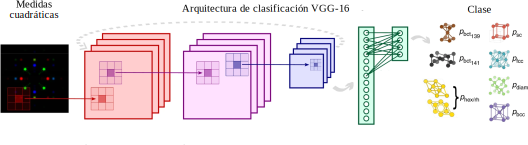
\includegraphics[height=0.25\textheight]{images/marco_teórico/crystal_clasification.pdf}
    \end{figure}
\end{frame}

\begin{frame}{Limitaciones}
\scriptsize
%Generalización de el esquema de clasificación para cada campo de propagación
    \begin{figure}
        \centering
        \includegraphics[width=0.6\linewidth]{images/marco_teórico/esquema_entrenamiento_tradicional2.pdf}
    \end{figure}
    \begin{itemize}
        %\item Se utiliza la red de clasificación sobre las medidas simuladas.
        \item El esquema \textbf{no tiene en cuenta el modelo de propagación} del campo óptico.
        \item Los trabajos realizados \textbf{no han estudiado los enfoques de clasificación para todos los campos de difracción}
        \item Hasta el momento, \textbf{no se ha estudiado la clasificación sobre medidas cuadráticas codificadas}.
    \end{itemize}
\end{frame}




\section{Metodología}
\begin{frame}{Objetivos}
\scriptsize
\begin{block}{\small Objetivo general}
Desarrollar un algoritmo de clasificación de objetos en imágenes difractivas basado en medidas cuadráticas codificadas usando un enfoque de aprendizaje profundo.

\end{block}
\begin{block}{\small Objetivos específicos}
\scriptsize
\begin{enumerate}

    \item \textbf{Modelar matemáticamente} el proceso de adquisición de medidas cuadráticas codificadas utilizando máscaras de fase.

    \item \textbf{Diseñar e implementar un algoritmo de clasificación} de objetos en medidas cuadráticas codificadas a partir de aprendizaje profundo que incorpore el modelo de adquisición.
    
    \item \textbf{Simular una configuración óptica difractiva para la adquisición de medidas cuadráticas codificadas} usando máscaras de fase.
    
    \item \textbf{Evaluar el algoritmo de clasificación de medidas cuadráticas codificadas} basado en aprendizaje profundo frente a otras técnicas del estado del arte usando medidas adquiridas con la configuración óptica simulada.

\end{enumerate}
\end{block}
\end{frame}

\begin{frame}{Enfoque de clasificación propuesto\footnote{\tiny Morales, D., et al. (2021). "Object Classification using Deep Neural Networks from Coded Diffraction Patterns".}}
\scriptsize
\begin{block}{ {\small Objetivo general y Objetivo específico 2} \checkmark}
\begin{figure}
    \centering
    \includegraphics[width=\linewidth]{images/metodología/esquema_entrenamiento.pdf}
\end{figure}
\vspace{-0.2cm}

\end{block}
% \begin{block}{Objetivos específicos}
% \begin{enumerate}

%     \item Modelar matemáticamente el proceso de adquisición de medidas cuadráticas codificadas utilizando máscaras de fase.

%     \item Diseñar e implementar un algoritmo de clasificación de objetos en medidas cuadráticas codificadas a partir de aprendizaje profundo que incorpore el modelo de adquisición.
    
%     \item Simular una configuración óptica difractiva para la adquisición de medidas cuadráticas codificadas usando máscaras de fase.
    
%     \item Evaluar el algoritmo de clasificación de medidas cuadráticas codificadas basado en aprendizaje profundo frente a otras técnicas del estado del arte usando medidas adquiridas con la configuración óptica simulada.

% \end{enumerate}
% \end{block}
\end{frame}

\begin{frame}{Estimación inicial}
\scriptsize
\vspace{-0.5cm}
\begin{figure}
    \centering
    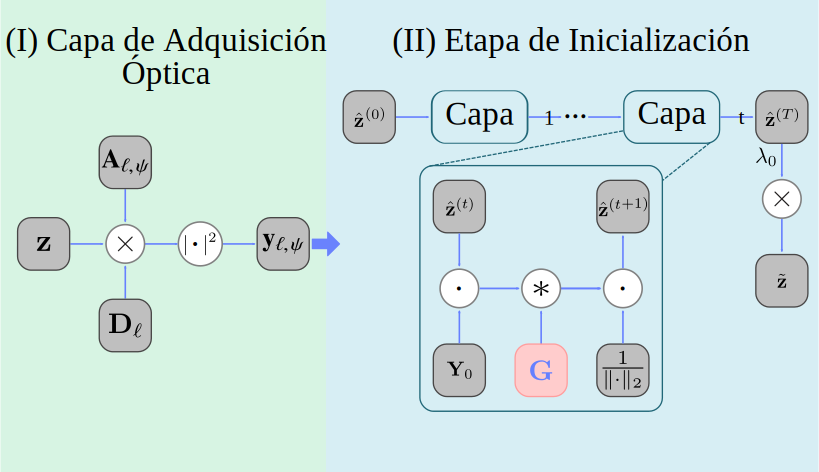
\includegraphics[width=0.6\linewidth]{images/metodología/inicialización.pdf}
\end{figure}
\vspace{-0.5cm}
\begin{block}{\small Problema de optimización}
\vspace{-0.5cm}
\begin{equation}
    \tilde{\mathbf{z}}\in\argmax_{\Vert{\mathbf{z}}\Vert_2=1}{\mathbf{z}}^\mathcal{H}\mathbf{Y}_{0}{\mathbf{z}}.
\end{equation}
\end{block}

\begin{itemize}
        \item Se incluye la modulación $\mathbf{D}_\ell$ y la matriz de sensado $\mathbf{A}_{\ell, \phi}$ en la etapa (I) cumpliendo con \textcolor{DarkGreen}{ Obj 1, 3 \checkmark}
        \item El filtro $\mathbf{G}$ se incluye como parámetros entrenables de la red neuronal
\end{itemize}
\end{frame}

\begin{frame}{Algoritmo LFSI \footnote{\tiny Morales D, et al. (2021) "Deep Phase Retrieval by a Learnable Filtered Spectral Initialization"}$^,$\footnote{\tiny Morales D, et al. (2021) "Learning spectral initialization for phase retrieval via deep neural networks"}}
\vspace{-0.6cm}
\scriptsize
\centering
\begin{algorithm}[H]
    %\renewcommand*{\linenosize}\tiny}
    %\algsetup{linenosize=\tiny}
    \scriptsize
    \caption{Inicialización Espectral Filtrada Aprendida (LFSI)}\label{fsi_algo}
    \begin{algorithmic}[1]
        \State{\textbf{Entrada:} Matriz de sensado y muestras $\{(\mathbf{A}_{\ell,\psi};\mathbf{y}_{\ell,\psi})\}_{\ell=1}^L$, máximo número de iteraciones $T$, filtro $ \mathbf{G}\in\mathbb{C}^{g\times g}$.}
		\State{$\hat{\mathbf{z}}\leftarrow$ Escogido aleatoriamente.}
		\State{\textbf{Asignar }$\Xi$ como el conjunto de índices correspondientes a los valores más grandes de $\{(\mathbf{y})_i / \Vert \mathbf{a}_{i,\psi}\Vert_{2}\}$.}
		\State{$$\mathbf{Y}_{0}:=\frac{1}{\mathrm{card}(\Xi_0)}\sum_{i\in\Xi}\frac{\mathbf{a}_{i,\psi}\mathbf{a}_{i,\psi}^\mathcal{H}}{\Vert\mathbf{a}_{i,\psi}\Vert_2^2}$$}
		\For{$t=0:T-1$} 
		\State{$\grave{\mathbf{z}}^{(t+1)}= \textcolor{red}{\mathbf{G}}*\left(\mathbf{Y}_{0}\hat{\mathbf{z}}^{(t)}\right).$\Comment{Filtrado}}
		\State{$\hat{\mathbf{z}}^{(t+1)}=\frac{\grave{\mathbf{z}}^{(t+1)}}{\left \| \grave{\mathbf{z}}^{(t+1)} \right \|_2}$}.		\Comment{Normalización}
		\EndFor
		\State{Compute $\tilde{\mathbf{z}} = \lambda_0\hat{\mathbf{z}}^{(T)}$.\Comment{Escalado}}
		%		\State{Compute $\mathbf{z}_{1}=\mathcal{A}(\mathbf{z}_{0})$\Comment{Denoising step}}
		\State{\textbf{salida: } Estimación inicial del campo óptico $\tilde{\mathbf{z}}$.}
	\end{algorithmic}
    \label{alg_1}
\end{algorithm}
\vspace{-0.4cm}
\begin{itemize}
    \scriptsize
    \item $\Xi$ corresponde al conjunto de índices asignados a los valores más grandes de $\{(\mathbf{y})_i / \Vert \mathbf{a}_{i,\psi}\Vert_{2}\}$ con $\mathbf{y}=[\mathbf{y}_{1,\psi}^\mathcal{T},\cdots,\mathbf{y}_{L,\psi}^\mathcal{T}]^\mathcal{T}$
    \item $\lambda_0$ es el factor de escala $\lambda_0=\sqrt{\sum_{\ell=1}^{L}\frac{\Vert\mathbf{y}_{\ell,\psi}\Vert_{2}^2}{nL}}$ .
    \vfill
\end{itemize}

\end{frame}

\subsection{Entrenamiento de extremo a extremo}
\begin{frame}{Entrenamiento de extremo a extremo}
\tiny
\begin{equation}
\mathbf{\theta}^*, \mathbf{G}^* \in  \argmin_{\mathbf{\theta}} \frac{1}{K}\sum_{k = 1}^{\mathcal{K}} \mathcal{L}\left( c^{(k)}, f_\theta(\mathrm{LFSI}\left(\mathbf{A}_{\ell,\psi},\mathbf{y}_{\ell, \psi}^{(k)}\right)\right) + \mathcal{I}(G).
\end{equation}

$$ \mathcal{I}_{\Omega}(\mathbf{G})=  \left\{\begin{matrix}
 0& \text{si } \mathbf{G}\in \Omega \\ 
+\infty & \text{si } \mathbf{G}\notin \Omega 
\end{matrix}\right. \quad \text{Con, }\quad \Omega=\{\mathbf{G}\in\mathbb{C}^{g\times g}| |(\mathbf{G})_{p,q}|\leq 1\}$$



\begin{algorithm}[H]
        %\algsetup{linenosize=\tiny}
        %\algsetup{linenosize=\tiny}
        \caption{\scriptsize Algoritmo de entrenamiento del esquema propuesto.   }
            \label{alg:algoritmo_2}
        	\begin{algorithmic}[1]
            \State{\textbf{Entrada:} Conjunto de entrenamiento $\{\mathbf{z}^{(k)}, {\mathbf{c}}^{(k)}\}_{k=1}^\mathcal{K}$ con $\mathcal{K}$ imágenes.}  
            \State{\textbf{Inicialización filtro:} {
            $\mathbf{G}\in \mathcal{U}(\mathbf{0},\mathbf{1})^{5 \times 5}$} }
            \For{época = 1:$\mathcal{E}$}\Comment{$\mathcal{E}$ épocas}
                \For{$k= 1$:$\mathcal{K}$}\Comment{$\mathcal{K}$ ejemplos}
                    \State{$\mathbf{y}_{\ell,\psi} = \vert \mathbf{A}_{\ell,\psi}\mathbf{z}^{(k)}\vert^2, \quad \ell\in\{1,\dots,L\}$}
                    \Comment{Médidas cuadráticas codificadas.}
                    \State{$\tilde{\mathbf{z}}^{(k)} \leftarrow  { \mathrm{LFSI}\left(\mathbf{A}_{\ell,\psi},\mathbf{y}_{\ell, \psi}\right)}$}\Comment{Algoritmo \ref{alg_1}}
                    %\State{$\hat{\mathbf{c}}^{(k)} \leftarrow  f_{\boldsymbol{\theta}}\left(\tilde{\mathbf{z}}^{(k)}\right)$}\Comment{Bloque de clasificación}
                    \State{$\mathcal{L}_{\mathbf{G},\boldsymbol{\theta}}=\frac{1}{\mathcal{K}}\sum_{k=1}^{\mathcal{K}} \mathcal{L}\left( c^{(k)},f_{\boldsymbol{\theta}}\left(\tilde{\mathbf{z}}^{(k)}\right) \right) $}    
               \Comment{Función de costo}     
                    \State{$\mathbf{G}\leftarrow\mathcal{A}_{dam}( \mathbf{G}, \beta_1 \nabla_{\mathbf{G}} \mathcal{L}_{\mathbf{G},\boldsymbol{\theta}}) $}    
                \Comment{Optimización sobre $\mathbf{G}$ }
                      \State{$\boldsymbol{\theta}\leftarrow\mathcal{A}_{dam}( \boldsymbol{\theta}, \beta_2 \nabla_{\boldsymbol{\theta}} \mathcal{L}_{\mathbf{G},\boldsymbol{\theta}}) $}    
                \Comment{Optimización sobre $\boldsymbol{\theta}$ }
                \EndFor
                \EndFor
		\State{\textbf{Salida: } Kernel óptimo $\mathbf{G}$ y parámetros de la red neuronal $\boldsymbol{\theta}$.}
	\end{algorithmic}
	%\label{alg:algoritmo_2}
\end{algorithm}
\end{frame}

\section{Simulaciones y resultados}
\subsection{Conjuntos de datos}
\begin{frame}{Conjuntos de datos}
    \scriptsize
    \begin{figure}
        \centering
        
\includegraphics[width=0.8\linewidth]{images/metodología/datasets.pdf}
        \label{fig:my_label}
    \end{figure}
    \begin{table}[!h]
    \renewcommand*{\arraystretch}{1.1}
    \centering\scalebox{0.7}{
    \resizebox{\textwidth}{!}{%
    \begin{tabular}{|c|c|c|c|c|}
    \hline
    \textbf{Conjunto de datos} & \textbf{Entrenamiento} & \textbf{Validación} & \textbf{Prueba} & \textbf{Total} \\ \hline
    MNIST                      & 54000                  & 6000                & 10000           & 70000          \\ \hline
    Fashion-MNIST              & 54000                  & 6000                & 10000           & 70000          \\ \hline
    \end{tabular}%
    }}
    \label{tab:conjunto_datos}
    \end{table}
    \begin{itemize}
        \item Actualmente no se encontraron conjuntos de datos públicos enfocados en la clasificación de medidas cuadráticas. Por esto, se usaron los conjuntos MNIST \footnote{\tiny Deng, Li (2012). "The mnist database of handwritten digit images for machine learning research".} y Fashion-MNIST\footnote{\tiny Han Xi et al (2017), "Fashion-mnist: a novel image dataset for benchmarking machine learning algorithms".}
        \item Cada imagen fue re dimensionada a $128 \times 128$ píxeles y escalada en el rango de $[0, 2\pi]$ para simular la información de fase $\boldsymbol{\varphi}$, en la entrada del algoritmo de la forma $\mathbf{z} = e^{(j \boldsymbol{\varphi})}$.
    \end{itemize}
\end{frame}

\subsection{Métricas}
\begin{frame}{Métricas para evaluar la inicialización}
    \centering
    \scriptsize \vspace{-0.5cm}
    \begin{block}{\scriptsize {\small \textcolor{red}{$\uparrow$}} Medida del índice de similitud estructural (SSIM), $ \in [0,1]$ }
    \begin{equation*}
        %\nonumber
        \mathrm{SSIM}(\mathbf{z}, \tilde{\mathbf{z}}) = \frac{2(\mu_{\mathbf{z}}\mu_{\tilde{\mathbf{z}}} + C_1) + (2\sigma_{\mathbf{z}\tilde{\mathbf{z}}} + C_2)}{(\mu_{\mathbf{z}} + \mu_{\tilde{\mathbf{z}}} + C_1)(\sigma_{\mathbf{z}}\sigma_{\tilde{\mathbf{z}}} + C_1)},
        \label{eq:SSIM}
    \end{equation*}
    \end{block}
    \begin{block}{\scriptsize {\small \textcolor{red}{$\uparrow$}} Relación de señal a ruido máxima (PSNR),$ \in [0,\infty)$}
    \begin{equation*}
        %\nonumber
        \mathrm{PSNR}(\mathbf{z}, \tilde{\mathbf{z}})=10 \cdot \log_{10}\left(\frac{\mathrm{MAX}^{2}}{\mathrm{MSE}(\mathbf{z}, \tilde{\mathbf{z}})}\right),
        \label{eq:PSNR}
    \end{equation*}
    \end{block}
    \begin{block}{\scriptsize {\small \textcolor{red}{$\downarrow$}} Error cuadrático medio (MSE) $[0,\infty)$}
    \begin{equation*}
        %\nonumber
        \mathrm{MSE}(\mathbf{z}, \tilde{\mathbf{z}}) = \frac{1}{n} \Vert \mathbf{z} - \tilde{\mathbf{z}}\Vert_2^2.
        \label{eq:MSE}
    \end{equation*}
    \end{block}
    \begin{block}{\scriptsize {\small \textcolor{red}{$\downarrow$}} Error relativo (RE) $[0,\infty)$}
        \begin{equation*}
            %\nonumber
            \mathrm{RE}(\mathbf{z}, \tilde{\mathbf{z}}) = \frac{ \mathrm{dist}(\mathbf{z}, \hat{\mathbf{z}})}{\Vert \mathbf{z} \Vert_2}.
            \label{eq:RE}
        \end{equation*}
    \end{block}

\end{frame}

\begin{frame}{Métricas para evaluar la clasificación}
    \centering
    \scriptsize \vspace{-0.5cm}
    \begin{block}{\scriptsize {\small \textcolor{red}{$\uparrow$}} Exactitud $ \in [0,1]$}
        \begin{equation*}
            \mathrm{Exactitud} = \frac{TP+TN}{TP+TN+FP+FN}.
        \end{equation*}
    \end{block}
    \begin{block}{\scriptsize {\small \textcolor{red}{$\uparrow$}} Precisión $ \in [0,1]$}
        \begin{equation*}
            \mathrm{Precisi\acute{o}n} = \frac{TP}{TP+FP}.
        \end{equation*}
    \end{block}
    \begin{block}{\scriptsize {\small \textcolor{red}{$\uparrow$}} Exhaustividad$ \in [0,1]$}
        \begin{equation*}
            \mathrm{Exhaustividad} = \frac{TP}{TP+FN}.
        \end{equation*}
    \end{block}
    \begin{block}{\scriptsize {\small \textcolor{red}{$\uparrow$}} Métrica F1 $\in [0,1]$}
        \begin{equation*}
            \mathrm{F1} = \frac{2\cdot\mathrm{Precisi\acute{o}n}\cdot\mathrm{Exhaustividad}}{\mathrm{Precisi\acute{o}n}+\mathrm{Exhaustividad}}.
        \end{equation*}
    \end{block}
    \vfill
    
    $TP$: Verdaderos positivos, \quad $TN$: Verdaderos negativos, \quad $FP$: Falsos positivos, \quad $FN$: Falsos negativos
\end{frame}

\subsection{Parámetros de los experimentos}


\begin{frame}{Parámetros de los experimentos}
\scriptsize
\vspace{-1cm}
\begin{block}{\scriptsize Parámetros modelos de clasificación}
    
    \begin{table}[!h]
    \centering
    \begin{tabular}{|c|c|c|}
    \hline
    \textbf{Modelo}      & \textbf{Número de parámetros} & \textbf{Número de capas} \\ \hline
    MobileNetV2 & 3,538,984            & 53              \\ \hline
    InceptionV3 & 23,851,784           & 48              \\ \hline
    Xception    & 22,910,480           & 71              \\ \hline
    \end{tabular}
    
    \end{table}
\end{block}
\vspace{-0.5cm}
\begin{block}{\scriptsize Parámetros modelos de propagación.}
\begin{table}[!h]
\centering
\renewcommand*{\arraystretch}{1.1}
\scalebox{0.9}{
\begin{tabular}{|l|r|r|c|}
\hline
\multicolumn{1}{|c|}{\textbf{Parámetros ópticos}} & \multicolumn{1}{c|}{\textbf{Campo cercano}} & \multicolumn{1}{c|}{\textbf{Campo medio}} & \textbf{Campo lejano} \\ \hline
Longitud de onda ($\lambda$) [nm]                    & 635                           & 635                            & -         \\ \hline
Distancia de propagación ($z$) [cm]         &    2.5                       & 7                              & -         \\ \hline
\end{tabular}}

\end{table}
\end{block}
\vspace{-0.5cm}
\begin{block}{\scriptsize Parámetros entrenamiento}
\scriptsize
\begin{itemize}
    \item Tamaño del filtro $\mathbf{G} \in \mathbb{C}^{g\times g}, g = 5$
    \item Se usó el algoritmo Adam con número de épocas $\mathcal{E}=100$ y tasa de aprendizaje $10^{-3}$
\end{itemize}   
\end{block}
\end{frame}


\begin{frame}{Comparaciones. Objetivo 4. \textcolor{DarkGreen}{\checkmark}}
    \scriptsize
    %\vspace{-1.5cm}
    \begin{block}{\scriptsize Comparación estimación inicial}
     
    \begin{itemize}
            \item \textit{Orthogonality promoting initialization} (OPI).
            \item \textit{Weighted Maximal Correlation Initialization} (WMCI).
            \item \textit{Filtered Spectral Initialization} (FSI).
        \item Estimación inicial aprendida (LFSI, Propuesto)
    \end{itemize}
    \end{block}
    %\vspace{-1cm}
    \begin{block}{\scriptsize Comparación clasificación. Objetivo específico 4}
    \begin{itemize}
        \item Esquema tradicional (Sin realizar estimación inicial.) \hfill
        $  \hat{c} = f_\theta\left(\mathbf{y}_{\ell, \psi} \right)$
        \item Usando algoritmo una estimación inicial aprendida ($\mathrm{LFSI}$, Propuesto). \hfill
        $ \hat{c} = f_\theta\left( \mathrm{LFSI}\left(\mathbf{A}_{\ell,\psi},\mathbf{y}_{\ell, \psi}\right) \right)
        $
        \item Empleando el modelo de propagación inverso (BPM, Propuesto). \hfill 
        $\hat{c} = f_\theta\left( \frac{1}{L}\sum_{\ell=1}^{ L} \mathbf{A}_{\ell, \psi}^{-1}\mathbf{y}_{\ell, \psi} \right).$
    \end{itemize}
        
    \end{block}
    
\end{frame}

\subsection{Simulaciones y resultados de la estimación inicial}
\begin{frame}{Resultados de la inicialización variando zona de difracción}
    \begin{figure}
        \centering
        \includegraphics[width=\linewidth]{images/resultados/results_initializations.pdf}
    \end{figure}
\end{frame}


\begin{frame}{Resultados de la inicialización variando el ruido}
    \begin{figure}
        \centering
        \includegraphics[height=0.75\textheight]{images/resultados/Noisy_Initializations.pdf}
    \end{figure}
\end{frame}

\begin{frame}{Resultados visuales de la inicialización.}
    \vfill    
    \begin{figure}
        \centering
        \includegraphics[width=\linewidth]{images/resultados/visual_cercano.pdf}
    \end{figure}
    \vfill
\end{frame}

\begin{frame}{Resultados visuales de la inicialización.}
    \vfill    
    \begin{figure}
        \centering
        \includegraphics[width=\linewidth]{images/resultados/visual_medio.pdf}
    \end{figure}
    \vfill
\end{frame}

\begin{frame}{Resultados visuales de la inicialización.}
    \vfill    
    \begin{figure}
        \centering
        \includegraphics[width=\linewidth]{images/resultados/visual_lejano.pdf}
    \end{figure}
    \vfill
\end{frame}

\subsection{Simulaciones y resultados de la clasificación}

\begin{frame}{Clasificación usando MobilnetV2}
\scriptsize
    \begin{figure}
        \centering
        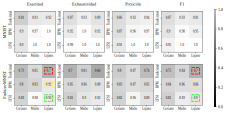
\includegraphics[width=\linewidth]{images/resultados/test_result_mobilnet.pdf}
    \end{figure}
\end{frame}

\begin{frame}{Clasificación usando InceptionV3}
\scriptsize
    \begin{figure}
        \centering
        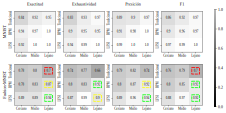
\includegraphics[width=\linewidth]{images/resultados/test_result_inception.pdf}
    \end{figure}
\end{frame}

\begin{frame}{Clasificación usando Xception}
\scriptsize
    \begin{figure}
        \centering
        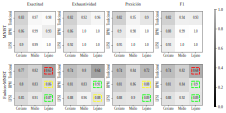
\includegraphics[width=\linewidth]{images/resultados/test_result_xception.pdf}
    \end{figure}
\end{frame}


\section{Conclusiones}
\begin{frame}{Conclusiones}
    \scriptsize
        \begin{block}{\scriptsize Inicialización}
        \begin{itemize}
            \item La inicialización propuesta permite estimar una aproximación en solo 10 iteraciones y una proyección.
            \item Incluir la etapa de la inicialización brinda robustés al algoritmo de clasificación.
        \end{itemize}
        \end{block}
        
        \begin{block}{\scriptsize Clasificación sobre medidas cuadráticas codificadas}
            \begin{itemize}
                \item La clasificación de medidas cuadráticas tiene comportamiento en los campos de difracción lejano y medio.
                \item El método propuesto supera al esquema de clasificación tradicional en 0.22 en la métrica F1 usando la red Inception V3.
            \end{itemize}        
        \end{block}


        \begin{block}{\scriptsize Trabajo de grado}
            \begin{itemize}
            \item Los ebjetivos planteados en este trabajo de grado fueron superados correctamente, por lo que se culminó exitosamente con este proyecto.
            \end{itemize}        
        \end{block}


\end{frame}

\begin{frame}{Trabajo futuro}
    \scriptsize
    \begin{block}{\scriptsize Validación}
        \begin{itemize}
            \item El método propuesto puede llegar a ser validado experimentalmente mediante la implementación de un sistema óptico de adquisición de medidas cuadráticas codificadas. 
            \end{itemize}
    \end{block}        
    \begin{block}{\scriptsize Entrenamiento de $\mathbf{D}_\ell$}
        \begin{itemize}
            \item Incluir una máscara de codificación $\mathbf{D}_\ell$ como pesos entrenables dentro del esquema de red neuronal, con el objetivo de determinar una codificación óptima que mejore el proceso de clasificación.
        \end{itemize}
    \end{block}
        
\end{frame}

\begin{frame}{Producción Académica}
    \begin{figure}
        \centering
        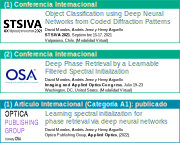
\includegraphics[height=0.75\textheight]{images/productos_tesis.pdf}
    \end{figure}
\end{frame}




\setLayout{blank}
\begin{frame}
    \centering
    \vspace{3cm}
    \textbf{\Huge ¡Gracias!}
    \ \\
    \textbf{Espacio para las preguntas}
    \ \\
    
\end{frame}



\end{document}